\documentclass[a4paper, 11pt, twocolumn]{article}

\usepackage[T1]{fontenc}
\usepackage[utf8]{inputenc}
\usepackage[francais]{babel}
\usepackage{fancyhdr}
\usepackage{amsmath}
\usepackage{framed}
\usepackage[a4paper]{geometry}
\usepackage{varwidth}
\usepackage[babel = true]{csquotes}
\usepackage{multicol}
\usepackage{caption}
\usepackage{float}
\usepackage[squaren,Gray]{SIunits}
\usepackage{graphicx}
\usepackage{wrapfig}
\usepackage{pgfplots}
\pgfplotsset{compat=1.15}
\usepackage{tikz}
\usepackage[compatibility, european, betterproportions]{circuitikz}
\usetikzlibrary{circuits.ee.IEC}
\ctikzset{bipoles/thickness=1}
\usepackage{multirow}
\usepackage{numprint}



\usepackage{hyperref}
%\expandafter\def\expandafter\UrlBreaks\expandafter{\UrlBreaks%  save the current one
%  \do\a\do\b\do\c\do\d\do\e\do\f\do\g\do\h\do\i\do\j%
%  \do\k\do\l\do\m\do\n\do\o\do\p\do\q\do\r\do\s\do\t%
%  \do\u\do\v\do\w\do\x\do\y\do\z\do\A\do\B\do\C\do\D%
%  \do\E\do\F\do\G\do\H\do\I\do\J\do\K\do\L\do\M\do\N%
%  \do\O\do\P\do\Q\do\R\do\S\do\T\do\U\do\V\do\W\do\X%
%  \do\Y\do\Z}

\usepackage[usenames,dvipsnames,pdf]{pstricks}
\usepackage{epsfig}
\usepackage{pst-grad} % For gradients
\usepackage{pst-plot} % For axes
\usepackage[space]{grffile} % For spaces in paths
\usepackage{etoolbox} % For spaces in paths

\captionsetup{labelfont={bf, sc}, textfont=it, justification=centering}

\usepackage{newfloat}
\DeclareFloatingEnvironment[
    fileext=los,
    listname={Liste des blocs},
    name=Bloc,
    placement=tbhp,
]{bloc}
\renewcommand\thebloc{\texttt{B\arabic{bloc}}}
\DeclareFloatingEnvironment[
    fileext=los,
    listname={Liste des amplificateurs},
    name=Amplificateur,
    placement=tbhp,
]{ampli}
\renewcommand\theampli{\texttt{A\arabic{ampli}}}

\definecolor{colorTPT}{RGB}{200,17,59}

\author{\textsc{Étudiants :}\\
Anas Bouzafour, Antoine Gallet, Antonin Godard, Geert-Jan Huizing\\
\textsc{Encadrants :}\\
Eloi de Cherisey, Julien Gori, Chadi Jabbour\\}
\title{\textbf{\texttt{[PAF]}$\quad$Une guitare qui perd les pédales \\ Effet trémolo piloté par un accéléromètre}}

\makeatletter
\def\@maketitle{%
  \newpage
  \null
  \vskip 2em%
  \let \footnote \thanks
  
    {\LARGE\centering \@title \par}%
    
    \vskip 1.5em%
    \begin{center}
    \begin{tabular}{ll}
        \multirow{4}{1.8cm}{
\includegraphics[width=1.8cm]{logoTPT.pdf}} & \textsc{Étudiants :} \\
& Anas Bouzafour, Antoine Gallet, Antonin Godard, Geert-Jan Huizing  \\
& \textsc{Encadrants :}  \\
& Eloi de Cherisey, Julien Gori, Chadi Jabbour
    \end{tabular}
    \end{center}
    
    \begin{center}
    {\large \textit{2017 -- 2018}}
    \end{center}
  \par
  \vskip 1.5em}
\makeatother

\begin{document}

\maketitle

\begin{abstract}
    Ce Projet d'Application Final se centre sur la création de l'effet trémolo en guitare. Cet effet consiste à faire \enquote{trembler}, c'est-à-dire à faire varier de façon cyclique l'amplitude du signal d'entrée de la guitare. 
\end{abstract}

\begin{figure*}[p]
    \centering
    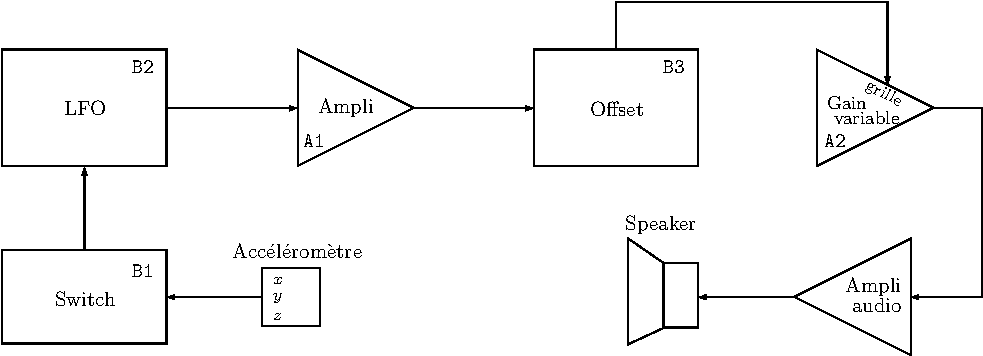
\includegraphics[width=\textwidth]{schema_bloc.pdf}
    \caption{Schéma principal du trémolo modulé par un accéléromètre}
    \label{fig:schemaBloc}
\end{figure*}

L'effet trémolo est un effet bien connu de la guitare électrique. Le principe du projet est de moduler l'amplitude du signal d'entrée de la guitare par une LFO (Low Frequency Oscillator) afin d'obtenir un effet de \enquote{vague}.

Pour coupler l'accéléromètre et l'effet du trémolo, nous avons décidé de faire varier la fréquence du LFO en fonction de la position du manche de la guitare où l'accéléromètre est fixé. Cela se décompose donc en deux étapes :
\begin{itemize}
    \item trouver une solution pour faire varier le gain d'entrée de la guitare ;
    \item réaliser un oscillateur à fréquence variable.
\end{itemize}

Nous nous référerons au schéma bloc (figure~\ref{fig:schemaBloc} page~\pageref{fig:schemaBloc}) afin de détailler chaque bloc de la chaîne de modulation du signal. Nous partirons du début de la chaîne de bloc (commutateur) jusqu'à la fin de la chaîne (amplificateur à fréquence variable).

\section{Commutateur pour régler la fréquence de l'oscillateur}

L'oscillateur figure~\ref{fig:oscillator} voit sa fréquence varier lorsque l'on change la valeur $R_4$ des résistances. Nous utilisons alors un montage commutateur afin d'activer ou non plusieurs résistances en série. Le schéma de montage est donné pour une des deux résistance de l'oscillateur, bloc~\ref{fig:commutateur} page~\pageref{fig:commutateur}. Ce montage permet donc de faire varier la fréquence de l'oscillateur par \enquote{palier}. En pratique, nous avons réalisé trois paliers de fréquence : $\sim 2\,\hertz$,  $\sim 4\,\hertz$, et  $\sim 6\,\hertz$.

Les coefficients $\alpha$ et $\beta$ sont à ajuster (on réalise un pont diviseur afin réduire / amplifier $V_\text{ref}$) afin que ces tensions de seuils comparées à $V_\text{capt}$ renvoyée par l'accéléromètre correspondent bien aux angles du manche de la guitare voulus. En pratique, nous avons fixé $V_\text{ref}$ à $\unit{1,6}{\volt}$ $\alpha V_\text{ref}$ à $\unit{1,4}{\volt}$. Nous obtenons donc trois \enquote{étages} de tension correspondant à trois fréquences selon la position du manche de la guitare.

\begin{bloc*}[p]
    \centering
    \shorthandoff{;:!?}
        \begin{circuitikz}[circuit ee IEC]
        \draw
            (-0.5,0) node[op amp](amp1){}
            (3,0) node[op amp](amp2){}
            (6.5,0) node[op amp](amp3){}
            
            (-2,3) to [*short] (-2,2.5) to [*R, l=$R_1$] ++(2,0) to [*R, l=$R_2$] ++(2,0)
                to [*R, l=$R_3$] ++(5,0)
                to [*R, l=$\ldots$] ++(2,0) -| ++(0.5,0.5)
                
            (0,2.5) to[*short, *-] ++(0,-1) to [*ospst] ++(2,0) to [*short, -*] ++(0,1)
            (3.5,2.5) to[*short, *-] ++(0,-1) to [*ospst] ++(2,0) to [*short, -*] ++(0,1)
            (7,2.5) to[*short, *-] ++(0,-1) to [*ospst] ++(2,0) to [*short, -*] ++(0,1)
        
            (amp1.out)  -| ++(0.36, 1.45)
            (amp2.out)  -| ++(0.36, 1.45)
            (amp3.out)  -| ++(0.36, 1.45)
            
            (-2.5,-1.5) node[circ](circ1){}
            (1.2,-1.5) node[circ](circ2){}
            (4.7,-1.5) node[circ](circ3){}
            
            (circ1) |- (amp1.-)
            (circ1) -- (circ2)
            (circ2) -- (circ3)
            (circ2) |- (amp2.-)
            (circ3) |- (amp3.-)
            (circ1) to [*short] ++(-0.5,0) node[left]{$V_\text{capt}$}
            
            (amp1.+) node[below]{\footnotesize $V_\text{ref}$}
            (amp2.+) node[below]{\footnotesize $\alpha V_\text{ref}$}
            (amp3.+) node[below]{\footnotesize $\beta V_\text{ref}$}
            
            ;
           
        \end{circuitikz}
    \shorthandon{;:!?}
    \caption{Résistance variable contrôlée par un commutateur}
    \label{fig:commutateur}
\end{bloc*}

\section{Un oscillateur à fréquence variable}

Nous avons premièrement réalisé un montage d'oscillateur bloc~\ref{fig:oscillator}. \`{A} l'alimentation, l'oscillateur subit un régime transitoire pendant lequel une sinusoïde rentre en régime instable, qui stabilise ensuite à l'aide d'un filtre de cette même fréquence. Il en résulte une sinusoïde d'amplitude constante $V_\text{osc}$, dont la fréquence est déterminée par la valeur des deux résistances de même valeur $R_4$ et dont la plage de fréquence désirée est de $1\,\hertz$ à $10\,\hertz$. C'est cette valeur de résistance que le Switch a pour rôle de faire varier. La résistance de valeur $R_5/2$ est en réalité une résistance variable, car son réglage précis est nécessaire afin d'obtenir ce régime sinusoïdal instable.

Le filtre réalisé est un passe-bande d'expression :

\begin{equation} \label{eq:osc}
    \frac{v_+}{V_\text{osc}} = \frac{1/3}{1 + Q(\frac{p}{\omega_0} + \frac{\omega_0}{p})}
\end{equation}

avec \[
    Q = \frac{1}{3}\quad \text{et}\quad \omega_0 = \frac{1}{R_4 C}
\]

Le caractère instable du filtre est assuré par la positivité (ou nullité) des pôles de la fonction de transfert.

\begin{bloc}
    \centering
    \shorthandoff{;:!?}
        \begin{circuitikz}[circuit ee IEC, scale=0.9]
        \draw
            
            (0,0) node[op amp](amp1) {}
            (amp1.+) node[left]{$v_+$} ++(0,0)
            % (-1,2) node[circ](circ2) {}
            
            (amp1.+) to [*short, -*] ++(0,-1.5)
            to [*tgeneric, l=$R_4$] ++(2,0) to [*C, l=$C_1$] ++(1,0) |- (amp1.out)
            
            (amp1.+) ++(0,-1.5) to [*short, -*] ++(-0.5,0)
            to [*short] ++(0,0.5) to [*C, a=$C_1$] ++(-1.5,0) to [*short, -*] ++(0,-0.5)
            (amp1.+) ++(-.5,-1.5) to [*short] ++(0,-0.5) to [*tgeneric, l=$R_4$] ++(-1.5,0) to [*short] ++(0,0.5)
            (-4.1,-2.05) node[ground]{} to [*short] ++(0.8,0)
            
            (amp1.-) to [*short, -*] ++(0,1)
            to [*R, a=$R_5/2$] ++(-2.4,0) to [*short] ++(0,-3.6)
            
            (amp1.-) ++(0,1) to [*R, l=$R_5$] ++(3,0) |- (amp1.out)
            
            (amp1.out) to [*short, -*] ++(1,0) node[right=0.1]{$V_\text{osc}$}
            
            ;
           
        \end{circuitikz}
    \shorthandon{;:!?}
    \caption{Oscillateur de tension}
    \label{fig:oscillator}
\end{bloc}

\section{Amplificateur inverseur et décalage à 1,2 V}

La tension de grille qui module le gain du trémolo a une plage de tension allant de $0,9\,\volt$ à $1,5\,\volt$, mais la sortie $V_\text{osc}$ est centrée en 0 et a une amplitude de $\,\volt$. On va donc réduire cette tension afin d'obtenir une amplitude de $300\,\milli\volt$ et décaler cette tension pour qu'elle soit centrée en $1,2\,\volt$. On utilise alors un amplificateur inverseur (amplificateur~\ref{fig:amplifierR}) dont les résistances $R_6$ et $R_7$ donnent un gain $-\frac{R_7}{R_6} = 0,15$.\footnote{Rappel : un amplificateur inverseur a pour fonction de transfert $\frac{V_s}{V_e} = -\frac{R_2}{R_1}$. De plus, inverser le signal ne s'entend pas à l'oreille.}

\begin{ampli}
    \centering
    \shorthandoff{;:!?}
        \begin{circuitikz}[circuit ee IEC, label = B1]
        \draw
            %l'ampli et le transistor
           (0,0) node[op amp](amp1) {}
           (0,2) node[resistor](R) {}
           
           %connexion de la masse
           (amp1.+) to ++(0,-1.5) node[ground, rotate =-90]{}
           
           %connexion des différents composants
           (amp1.-) to [*resistor, a=$R_6$] (-3,0.5) to ++(-.2,0) node[left=0.1]{$V_\text{osc}$}
           (amp1.-) |- (R)
           (R) -| (amp1.out)
           (R) ++(0,0.4) node[]{$R_7$}
           (amp1.out) to ++(0.3,0) node[right=0.1]{$V_\text{osc}'$}
           ;
           
        \end{circuitikz}
    \shorthandon{;:!?}
    \caption{Circuit amplificateur inverseur de tension}
    \label{fig:amplifierR}
\end{ampli}

La tension réduite $V_\text{osc}'$ est ensuite décalée avec le montage au bloc~\ref{fig:offset}. En approximant sur le gain de la fonction de transfert, on obtient :
\[
\frac{V_\text{mod}}{V_+} \simeq \frac{R_9}{R_8 + R_9}
\]

On veut également choisir une capacité afin de filtrer le signal à une fréquence très basse. Nous utilisons une capacité chimique car $\forall t\quad V_\text{mod} > V_\text{osc}'$, et nous filtrons à la fréquence $0,1\,\hertz$.

\begin{bloc}
    \centering
    \shorthandoff{;:!?}
        \begin{circuitikz}[circuit ee IEC]
        \draw
            (0,2) node[circ](circ1){}
            (0,4) node[circ](circ2){}
            (1,2) node[circ](circ3){}
            (-1.5,2) node[circ](circ4){}

           
            (0,0) node[ground, rotate=-90]{} to [*R, a=$R_9$] (0,2) to [*R, a=$R_8$] (0,4)
            (circ1) to [*ecapacitor, a=$C_2$] ++(-1.5,0) ++(-.3,0) node[left=0.1]{$V_\text{osc}'$}
            (circ1) to (circ3)
            (circ3) ++(0.3,0) node[right=0.1]{$V_\text{mod}$}
            (circ2) ++(0.3,0) node[above=0.1]{$V_+ = 15\,\volt$}
           ;
           
        \end{circuitikz}
    \shorthandon{;:!?}
    \caption{Réalisation d'un offset de $1,2\,\volt$}
    \label{fig:offset}
\end{bloc}

\section{Amplificateur inverseur à gain variable}

La solution que nous avons choisi est celle d'un montage amplificateur inverseur (ampli~\ref{fig:amplifierCMOS}) à résistance variable. La variation de la résistance entraîne la variation du gain. Ici, le transistor est équivalent à une résistance variable que nous appellerons $R_t$. Le gain de l'amplificateur est donc $-\frac{R_t}{R_{10}}$.

\begin{ampli}
    \centering
    \shorthandoff{;:!?}
        \begin{circuitikz}[circuit ee IEC]
        \draw
            %l'ampli et le transistor
           (0,0) node[op amp](amp1) {}
           (0,2) node[nmos, rotate=-90](nmos1) {}
           
           %connexion de la masse
           (amp1.+) to ++(0,-1.5) node[ground, rotate =-90]{}
           
           %connexion des différents composants
           (amp1.-) to [*R, a=$R_{10}$] (-3,0.5) to ++(-.2,0) node[left=0.1]{$V_e$}
           (amp1.-) |- (nmos1.E)
           (nmos1.C) -| (amp1.out)
           (nmos1.B) ++(0,0.3) node[]{$V_g$}
           (amp1.out) to ++(0.3,0) node[right=0.1]{$V_s$}
           ;
           
        \end{circuitikz}
    \shorthandon{;:!?}
    \caption{Circuit amplicateur de tension à gain variable}
    \label{fig:amplifierCMOS}
\end{ampli}

Une première étude de la valeur de la résistance $R_t$ était nécessaire au choix de $R_{10}$. On réalise un pont diviseur de tension afin d'isoler la résistance équivalente du transistor $R_t$ (figure~\ref{fig:mesureRt}).

\begin{figure}[H]
    \centering
    \shorthandoff{;:!?}
        \begin{circuitikz}[circuit ee IEC]
        \draw
            %l'ampli et le transistor
           (0,0) node[nmos](nmos1){}
           (1,-.5) to [*tfullgeneric, a=$R_t$, l=$\equiv$] (1,.5)
           (0,1) node[circ](circ1){}
           (-1.5,3) node[circ](circ2){}
           (1,1) node[circ](circ3){}
           (-1,0) node[circ](circ4){}
           
           (nmos1.B) ++(-0.3,0) node[]{$V_g$}
           (nmos1.E) to ++(0,-0.2) node[ground, rotate=-90]{}
           (nmos1.C) to (circ1) 
                to [*R, l=$R_\text{car}$] (0,3) 
                to (circ2) 
                to node[left=0.1]{$V_\text{DD}$} (-1.5,3)
           (circ1) to (circ3) to node[right=0.1]{$V_d$} (1,1)
           ;
           
        \end{circuitikz}
    \shorthandon{;:!?}
    \caption{Pont diviseur de tension pour la mesure de $R_t$}
    \label{fig:mesureRt}
\end{figure}

\begin{figure}
    \centering
    \begin{tikzpicture}
    \begin{axis}[
        width=7cm,
        grid=major,
        grid style = dashed,
        xlabel = $V_g\,(\volt)$,
        ylabel = $R_t\,(\ohm)$
        ]
        
        \addplot[mark = *, color = colorTPT] coordinates {
        
        (1.01,902911.111111113)
        (1.2,185196.226415095)
        (1.4,61056.7567567568)
        (1.6,24837.8726833199)
        (1.79,18475.3415744958)
        (2.01,6469.0518783542)
        (2.2,2011.70610211706)
        (2.39,935.472370766489)
        (2.59, 720.800696257615)
        (2.8, 605.841924398626)
        (3,	532.694355697551)

        };
        
    \end{axis}
    \end{tikzpicture}
    \caption{Mesure de $R_t$}
    \label{fig:RtVg}
\end{figure}

On obtient aisément l'équation :
\[
    R_t = R_\text{car}\frac{V_d}{V_{DD}-V_d}
\]

On obtient ainsi les valeurs de $R_t$ figure~\ref{fig:RtVg}. La courbe ayant une décroissance exponentielle, il faudra trouver la bonne valeur de $R_{10}$ afin de se placer dans une partie quasi-linéaire de la courbe pour obtenir une variation de gain quasi-linéaire. En pratique : $V_g \in \left[ 1\,\volt ; 1,6\,\volt \right]$.

\section*{Valeurs des composants des montages}

On donne ci-dessous à la table~\ref{tab:valeurs} les différentes valeurs des différents montages réalisés pour le projet.

\begin{table}[H]
    \centering
    \begin{tabular}{|c|c|}
    \hline
    Composant &  Valeur\\
    \hline\hline
    $R_1$ & $\unit{20}{\kilo\ohm}$\\
    \hline
    $R_2$ & $\unit{14}{\kilo\ohm}$\\
    \hline
    $R_3$ & $\unit{14}{\kilo\ohm}$\\
    \hline
    $R_5$ & $\unit{9,6}{\kilo\ohm}$\\
    \hline
    $R_6$ & $\unit{40,1}{\kilo\ohm}$\\
    \hline
    $R_7$ & $\unit{9,7}{\kilo\ohm}$\\
    \hline
    $R_8$ & $\unit{500}{\kilo\ohm}$\\
    \hline
    $R_9$ & $\unit{70,1}{\kilo\ohm}$\\
    \hline
    $R_{10}$ & $\unit{810}{\ohm}$\\
    \hline
    $C_1$ & $\unit{470}{\nano\farad}$\\
    \hline
    $C_2$ & $\unit{23}{\micro\farad}$\\
    \hline
\end{tabular}
    \caption{Tableau de valeurs des différents composants des montages}
    \label{tab:valeurs}
\end{table}


%\end{multicols*}

\end{document}
